%
\begin{figure*}[ht!]
    \centering
    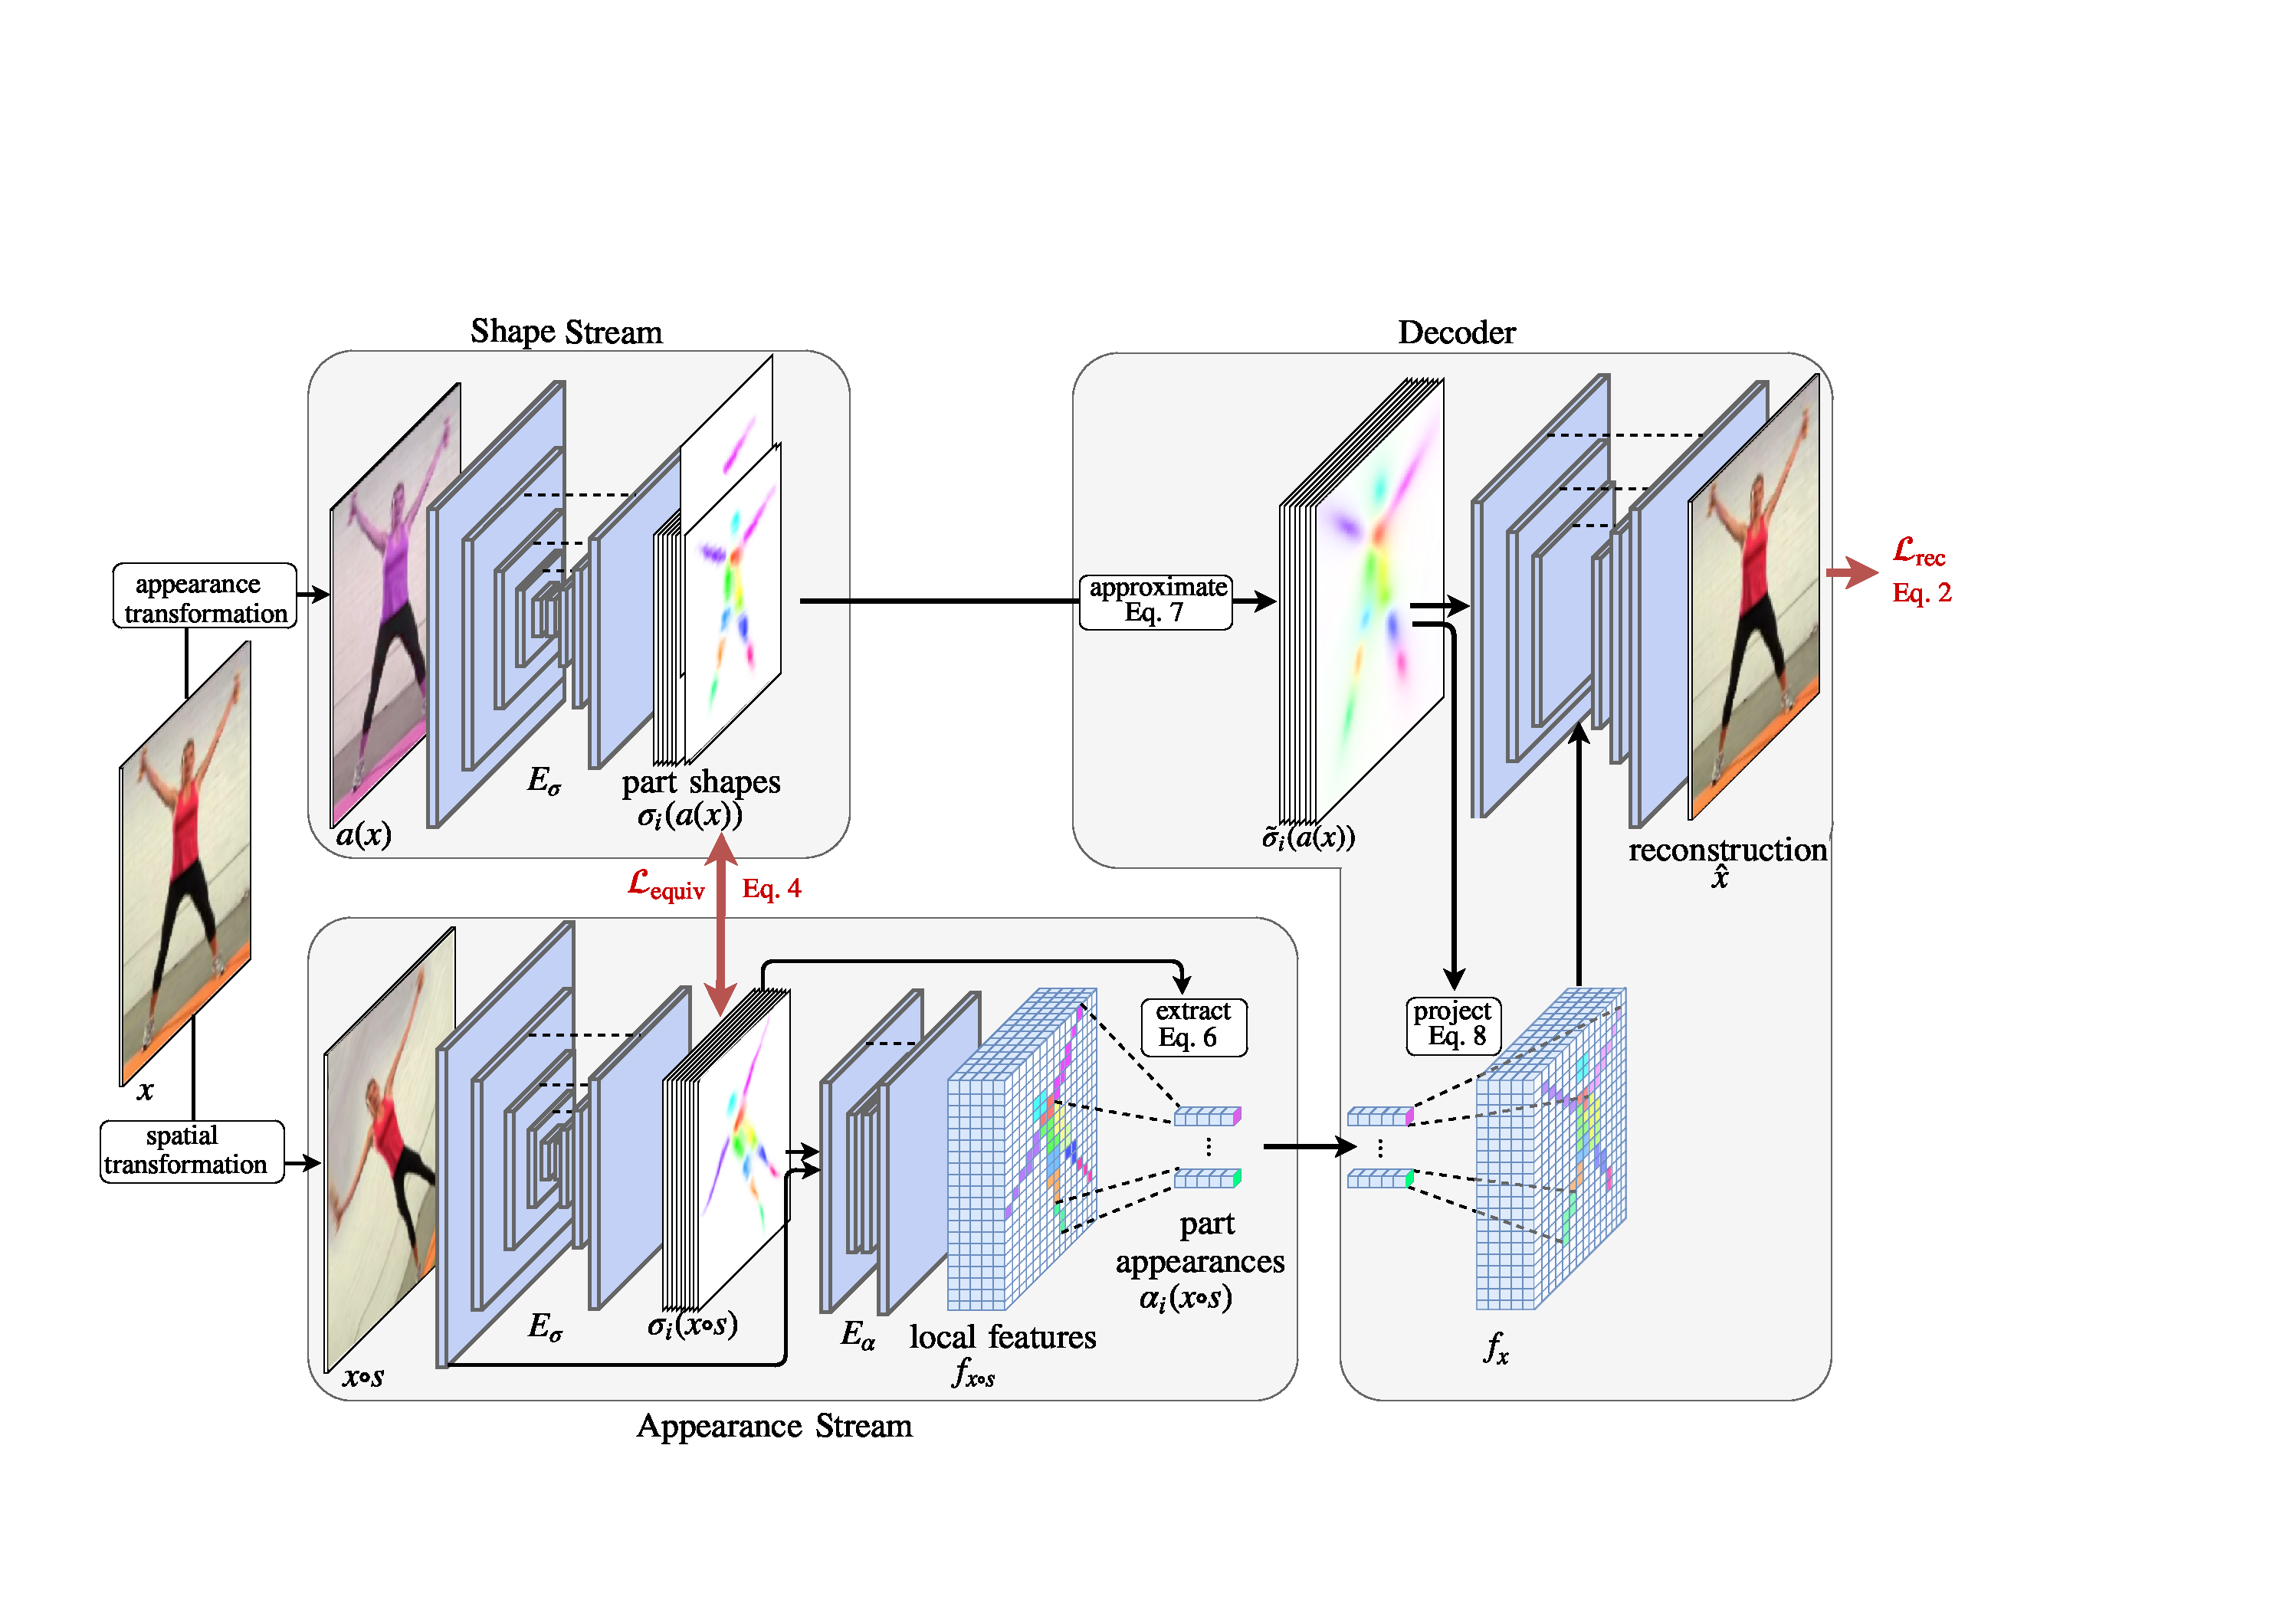
\includegraphics[trim={2cm 3cm 7cm 7cm},clip, width=0.97\linewidth]{fig/architecture_final.pdf}
	\caption{Two-stream autoencoding architecture for unsupervised learning of object shape and appearance.} %See Sect. \ref{sec:architecture} for details.}
    \label{fig:architecture}
\end{figure*}
%
\section{Approach}
    Let $x: \Lambda \rightarrow \mathbb{R}$ be an image portraying an object and background clutter. $\Lambda \subset \mathbb{N}^2$ is the space of image coordinates. Now consider an image $x': \Lambda \rightarrow \mathbb{R}$ showing another instance of the same object category. Despite drastic differences of their image pixels, you can recognize both to be related. What renders both images similar although no two pixels are identical? What are the characteristic, salient differences? And how can we obtain a representation $\phi$ that maps images to vectors $\phi(x)$ which retain both, these similarities and also the characteristic differences?
    %
\subsection{Part-based Representation}
    Numerous causes may have led $x$ to be changed into $x'$ (change in articulation, viewpoint, object color or clothing, lighting conditions, % clutter,
    etc.). But we can approximate and summarize their effects as a combination of a change in appearance and a change in shape.
    The effect of a change in object shape on an image $x$ can be expressed in terms of a spatial image transformation  $s: \Lambda \rightarrow \Lambda$ acting on the underlying image coordinates, such that the image $x {\circ} s$ depicts the object with altered shape.
    Similarly, we denote the effect of a change in object appearance on an image $x$ as an image transformation $a$ such that the image $a(x)$ depicts the object with altered appearance.

    Note that many of the image changes are local in nature, affecting only part of the image. For instance, animals may only move an individual body part. Similarly, only part of their appearance may vary, \eg, by switching a shirt but not the pants.
    This motivates a part-based factorization of the representation, $\phi(x):=( \phi_1(x), \phi_2(x), \dots )^\top$, so that local changes in appearance and shape stay local and do not alter the overall representation. Nevertheless, global changes can also be accounted for by representing them as as a composition of changes in the individual part representations $\phi_i$.

    %Nevertheless, global changes can also be modelled by altering all parts jointly. -> all parts? all part representations?
\subsection{Invariance and Equivariance}
    Let us now carefully observe differences between images $x$ and $x'$ to derive constraints for the representation $\phi$ that is to be learned.
    \emph{i)} Changes in the appearance of an object (\eg in its color or texture), should not impact its shape.
    \emph{ii)} Similarly, changes in shape (\eg through articulation), should not alter the appearance.
    Therefore, the representation needs to separate appearance and shape of the object, so that both can vary individually, i.e. the representation of a part is disentangled into two components $\phi_i(x)=(\alpha_i(x), \sigma_i(x))$.
    Part appearance is modeled as an $n$-dimensional feature vector $\alpha_i(x) \in \mathbb{R}^{n}$.
    Whereas part shape is modeled as a part activation map $\sigma_i(x): \Lambda \rightarrow \mathbb{R}^+$.
    We visualize these maps as colored images (cf. Fig. \ref{fig:architecture}, Fig. \ref{fig:shape}), where each color denotes a single part activation map.

    The invariance of our representation under changes in object appearance and shape can be summarized by the invariance constraints \emph{i)}
    $\alpha_i(x {{\circ}}s) = \alpha_i(x)$ and
    \emph{ii)} $\sigma_i(a(x)) = \sigma_i(x)$.
    In addition, changes in shape should obviously be captured by the shape representation. Thus, for spatial transformations $s$ we obtain the equivariance constraint \emph{iii)}
    $\sigma_i(x {{\circ}}s) = \sigma_i(x) {{\circ}}s$.
    The equivariance constraint simply states that the part activation maps have to consistently track the object part they represent (cf. $\sigma_i(a(x))$ and $\sigma_i(x {\circ} s)$ in Fig. \ref{fig:architecture}).

\subsection{Objective Function for Learning}
    Learning of the representation $\phi$ is driven by integrating invariance and equivariance constraints from the previous section into a reconstruction task.
    The invariance constraints \emph{i}) and \emph{ii}) imply
     \begin{equation}
    \phi_i(x) = [\alpha_i(x), \sigma_i(x)] \overset{!}{=}
    [\alpha_i(x {{\circ}}s), \sigma_i(a({x))]}.
    \label{eq:invarRep}
    \end{equation}
    Let $D([\phi_i(x)]_{i = 1, \dotsc,})$ be a reconstruction of the original image $x$ from the encoded part representations $\phi_1(x), \phi_2(x), ...$ using a decoder $D$. We seek to reconstruct $x$ and, simultaneously, demand the representation to obey the invariance constraints summarized in (\ref{eq:invarRep}),
    \begin{equation}
        \mathcal{L}_\text{rec} =
         \left\lVert x- D\left(\bigl[\alpha_i(x  {{\circ}}s), \sigma_i(a(x))\bigr]_{i = 1,\dotsc}\right)\right\rVert_1
        \label{eq:l_rec}
        .
    \end{equation}
    Moreover, the representation of part shape $\sigma_i(x)$ should be equivariant under deformations. However, simply minimizing equivariance on the scale of pixels, i.e.
    \begin{equation}
     \sum_i \sum_{u \in \Lambda} \Bigl\lVert \sigma_i(x {{\circ}}s)[u]- \sigma_i(x)[s(u)]\Bigr\rVert
     \label{eq:pixeleq}
	    ,
    \end{equation}
    is unstable in practice and favors to the trivial solution of uniform part activations.
    Therefore, we establish an equivariance loss % is based on the idea of matching the first moments of the part activations,
    \begin{equation}
    \begin{split}
    \mathcal{L}_{\textrm{equiv}} &= \sum_i \lambda_{\mu} \lVert  \mu[\sigma_i(x{{\circ}}s)]  - \mu[\sigma_i(a(x)) {{\circ}}s]\rVert_{2}  \\ &+ \lambda_{\Sigma} \lVert \Sigma[\sigma_i(x{{\circ}}s)] -  \Sigma[\sigma_i(a(x)) {{\circ}}s] \rVert_{1} \;,
    \end{split}
    \label{eq:equiv}
    \end{equation}
    where $\mu[\sigma_i(x)]$ and $\Sigma[\sigma_i(x)]$ denote the mean and covariance of
    $\sigma_i(x)/ \sum_{u \in \Lambda} \sigma_i(x)[u]$.
    Note that we have employed invariance \emph{ii)} so that we can use the same shape encoding $\sigma_i(a(x))$ as in (\ref{eq:l_rec}).
    The overall training objective of our model is to minimize the reconstruction and equivariance loss,
    \begin{equation}
        \mathcal{L} =  \mathcal{L}_\text{rec} + \mathcal{L}_\text{equiv}
        \label{eq:totalloss}
        .
    \end{equation}
    % TODOi
    %Note that we do not enforce invariance between parts. Thus, our model can learn relations between them.
    %Note that the parts are a priori unknown and there is no constraint on their placement or their mutual distances as in \cite{Zhang:2018vz, Thewlis:2017wi}, since this would entail a bias on part placement, cf. Sec. \ref{sec:shape}. Instead, the part representation (cf. sec. \ref{sec:architecture}) as disentangled components of shape and appearance is driven to cover the object in order to reconstruct it.
    Note that object parts a priori unknown, but in order to reconstruct the object, the representations $\phi_i$ automatically learn to structure it into meaningful parts which capture the variance in shape and appearance. In particular, we do not need to introduce artificial prior assumptions about the relations between parts, such as the separation constraints employed in \cite{Zhang:2018vz, Thewlis:2017wi}.
    Instead, the local modelling of the part representation (cf. sec. \ref{sec:architecture}) as disentangled components of shape and appearance drives our representation to meaningfully structure the object and learn natural relations between parts.

\subsection{Unsupervised Learning of Part-based Shape and Appearance}
    \label{sec:architecture}
    Subsequently, we discuss the network architecture in Fig. \ref{fig:architecture} for unsupervised learning of an appearance and shape representation using the reconstruction (\ref{eq:l_rec}) and equivariance loss (\ref{eq:equiv}).
    Learning considers image pairs $x {{\circ}} s$ and  $a(x)$.
    The leading design principle of our architecture is to model the local interplay between part shape and part appearance.
    In a fully differentiable procedure equivariance of part activation maps is used to extract part appearances from $x {{\circ}} s$ and assign them to corresponding image regions in $x$.


    \textbf{Part Shape.}
    In a shape stream (cf. Fig. \ref{fig:architecture}), an hourglass network \cite{Newell:2016vq} $E_{\sigma}$ learns to \emph{localize} parts $i$ by means of part activation maps $\sigma_i(a(x)) \in \mathbb{R}^{h\times w}$.
    The hourglass model nicely suits this task, since it preserves pixel-wise locality and integrates information from multiple scales \cite{Newell:2016vq}. Multi-scale context is essential to learn the relations between parts and consistently assign them to an object.
    %Note that the parts are a priori unknown and there is no constraint on their placement or their mutual distances as in \cite{Zhang:2018vz, Thewlis:2017wi}, since this would entail a bias on part placement, cf. Sec. \ref{sec:shape}.


    \textbf{Part Appearance.}
    Let us now localize the parts by detecting $\sigma_i(x {\circ} s)$ in a spatially transformed image $x {\circ} s$ using the same network $E_{\sigma}$ (cf. Fig. \ref{fig:architecture} Appearance Stream).
    To learn representations of part appearance $\alpha_i(x {\circ} s)$, we first stack all normalized part activations $\sigma_i(x {\circ} s)/\sum_{u \in \Lambda} \sigma_i(x {\circ} s)[u]$ and an image encoding, i.e., the output of the first convolution filters of the network $E_\sigma$ applied to $x{\circ} s$. A second hourglass network $E_{\alpha}$ takes this stack as input and maps it onto a localized image appearance encoding ${f_{x{\circ} s}} \in \mathbb{R}^{h\times w \times n}$. %To realize the local modelling of the part appearance we average pool ${f_{x{\circ} s}}$ at all locations where part $i$ has positive activation,
    To obtain local part appearances, we average pool these features at all locations where part $i$ has positive activation
    \begin{equation}
    \alpha_i(x {\circ} s) =
    \frac{ \sum_{u \in  \Lambda} f_{x{\circ} s}[u] \sigma_i(x {\circ} s)[u] }
    { \sum_{u \in  \Lambda} \sigma_i(x {\circ} s)[u] }
    \label{eq:appearance_encoding}.
    \end{equation}

    \textbf{Reconstructing the Original Image.}
    Next we reconstruct $x$ from part appearances %part appearance
    $\alpha_i(x {\circ} s)$ and %part activations shape descriptions
    part activations $\sigma_i(a(x))$ using a U-Net~\cite{Ronneberger:2015gk} (cf. Fig. \ref{fig:architecture}). The encoder of the U-Net is simply a set of fixed downsampling layers. Only its decoder is learned.
    We approximate part activations %shapes %
    $\sigma_i(a(x))$ by their
    first two moments,
    \begin{equation}
    \tilde{\sigma}_i(a(x))[u] = \frac{1}{1 + (u -\mu_i)^T \Sigma_i^{-1} (u - \mu_i)},
    \end{equation}
    where $\mu_i$ and  $\Sigma_i$ denote the mean and covariance of the normalized part activation maps $\sigma_i(a(x))/\sum_{u \in \Lambda} \sigma_i(a(x))[u]$. Thus, extra information present in part activations %$\sigma_i(a(x))$ %part activations
    is neglected, forcing the shape encoder $E_\sigma$ to concentrate on an unambiguous part localization (or else reconstruction loss would increase).
    The second input to the decoder $D$ in Eq.~\ref{eq:l_rec} are part appearances $\alpha_i(x{\circ} s)$.
    Note that $\alpha_i(x{\circ} s)$ are feature vectors devoid of localization.
    We exploit the fact that the corresponding part activations %part activation maps
     $\tilde{\sigma}_i(a(x))$ designate the regions of parts $i$ in image $x$ (cf. Fig \ref{fig:architecture}) to project the part appearances onto a localized appearance encoding $f_x$:
    \begin{equation}
        f_x[u]=  \sum_i
        \frac{ \alpha_i(x{\circ} s) \cdot \tilde{\sigma}_i(a(x))[u]}
        {1+ \sum_j \tilde{\sigma}_j(a(x))[u]}
        .
    \end{equation}
    To reconstruct $x$, the U-Net can then exploit the local correspondence between $f_x$,  $\tilde{\sigma}_i(a(x))$ and $x$.
   % Utilizing the local correspondences between $f_x$ , $\tilde{\sigma}_i(a(x))$ and the reconstruction target the U-Net decodes the image $x$.

\subsection{Implementation Details}
For appearance transformation $a$ we apply changes in brightness, contrast, and hue.
For image datasets, $s$ are thin plate spline (TPS) transformations.
On video datasets, in addition to applying synthetic TPS transformations we randomly sample another frame from the same video sequence which acts as $x {\circ} s$.
%
Selecting the number of parts is uncritical, since our model is robust for different numbers of parts, Tab. \ref{tab:static}.
%
For image synthesis in Sect. \ref{sec:dis} we train the decoder $D$ with an adversarial loss \cite{Isola2017image}.
We refer to the supplementary for further details on the architecture and the experimental setup.
